\documentclass{article}
\usepackage{tikz}
\usepackage{verbatim}
\usetikzlibrary{arrows,shapes}

\usepackage{coffee4}

\begin{document}
\title{LaTeX Coffee Stains}
\author{Hanno Rein\\
\texttt{http://hanno-rein.de}\\
Cambridge University}
\renewcommand{\today}{April 3, 2009}
\maketitle

\cofeAm{1}{1.0}{0}{5.5cm}{3cm}
 
\section{Introduction}
This package provides an essential feature to \LaTeX~that has been missing for too long. It adds a coffee stain to your documents. A lot of time can be saved by printing stains directly on the page rather than adding it manually. You can choose from four different stain types:
\begin{enumerate}
  \item $270^\circ$ circle stain with two tiny splashes 
  \item $60^\circ$ circle stain 
  \item two splashes with light colours
  \item and a colourful twin splash.
\end{enumerate}


\center{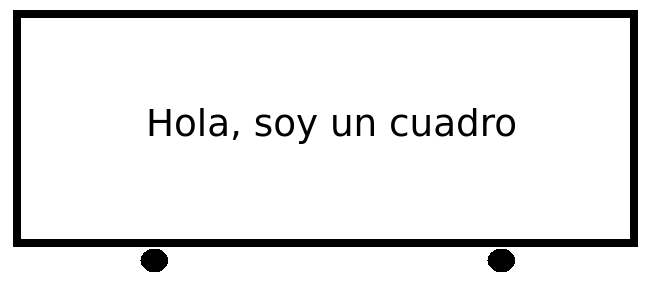
\includegraphics[scale=0.5]{images/soltrivial.png}}


\section{Usage}
To use the package, simply place the \texttt{coffee3.sty} file in the directory with all of your 
other \texttt{.tex} files \textit{or} install it properly (consult your distribution's manual). 
Then include the following line in the header of your document:
\begin{verbatim}
\usepackage{coffee4}
\end{verbatim}
To place a coffee stain on a page, put one of the following commands in the source code of the relevant page: 
\begin{verbatim}
\cofeAm{alpha}{scale}{angle}{xoff}{yoff}
\cofeBm{alpha}{scale}{angle}{xoff}{yoff}
\cofeCm{alpha}{scale}{angle}{xoff}{yoff}
\cofeDm{alpha}{scale}{angle}{xoff}{yoff}
\end{verbatim}
where alpha is the transparency factor $\in [0,1]$. The scale factor is {\tt scale}, and the standard is {\tt scale}=1. 
The angle is in degrees $\in [0,360]$. 
The position relative to the centre of the page is given by x and y offsets \texttt{xoff} and \texttt{yoff}.

\section{Copyright}
You can freely distribute this package as I do not believe in imaginary property. All stains are self-made, photographed by myself, processed with gimp and traced with Inkscape.
Donations should be made in coffee only. My address is
\begin{quote}
Hanno Rein\\
DAMTP, CMS\\
Wilberforce Road\\
Cambridge CB3 0WA\\
United Kingdom
\end{quote}
See more coffee stains on the next pages.
\cofeCm{0.9}{1}{180}{0}{0}
\newpage
\cofeDm{0.4}{0.5}{90}{0}{0}
Coffee is great.
\newpage
\cofeBm{0.7}{1}{0}{0}{0}
Coffee will save the world. 

\newpage
\cofeAm{0.7}{0.75}{2}{0}{0}
Coffee will save the world. 

\end{document}
